\documentclass{beamer}

\usepackage{graphicx,hyperref,udesc,url}
%\usepackage[latin1]{inputenc}
%\usepackage[T1]{fontenc}
\usepackage{listings}
\usepackage{booktabs}
\usepackage{bussproofs}
\usepackage{mathtools}
\usepackage[brazil]{babel}   
\usepackage[utf8]{inputenc}

\DeclarePairedDelimiter\ket{\lvert}{\rangle}

\title[Mini-Introdução à Teoria da Complexidade Quântica]{Mini-Introdução à\\ Teoria da Complexidade Quântica}

\author[Rafael Castro]{
    Rafael Castro\\\medskip
    {\small \url{rafaelcgs10@gmail.com}}}

\date{03 de Abril de 2019}

    \institute[UDESC]{
        Departamento de Ci\^encia da Computa\c{c}\~ao \\
            Centro de Ci\^encias e Tecnol\'ogicas\\
            Universidade do Estado de Santa Catarina}

\begin{document}

\begin{frame}
\titlepage

\end{frame}

\section{Introdução e Fundamentos}
\begin{frame}
\frametitle{Bettina}
\begin{figure}[h]
\label{bloch}
\centering
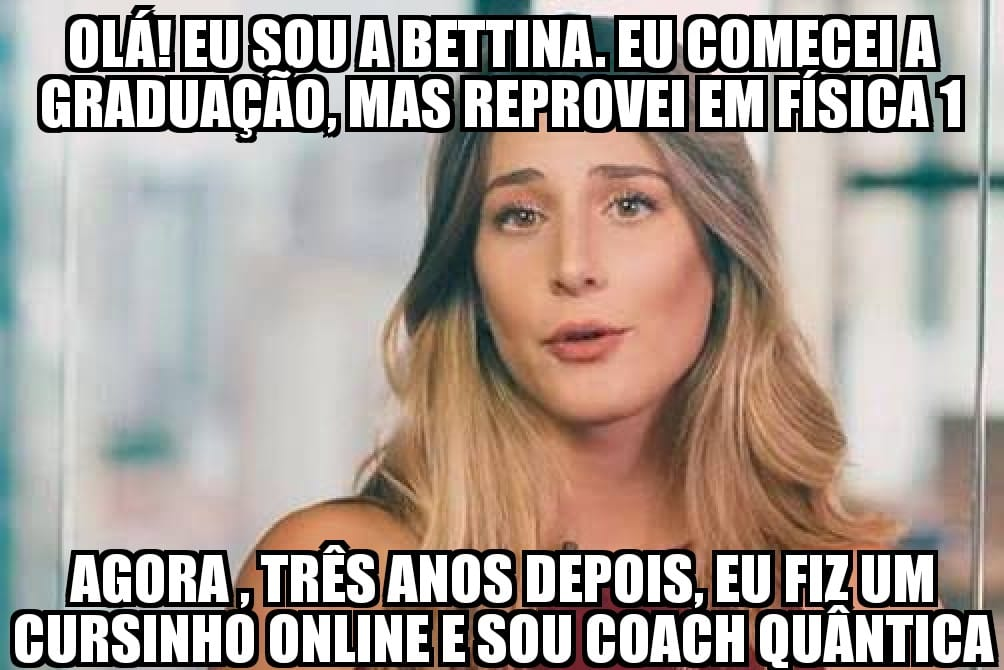
\includegraphics[width=0.8\textwidth]{betina.jpg}
\end{figure}
\end{frame}

\begin{frame}
\frametitle{Motivação}
\begin{figure}[h]
\label{bloch}
\centering
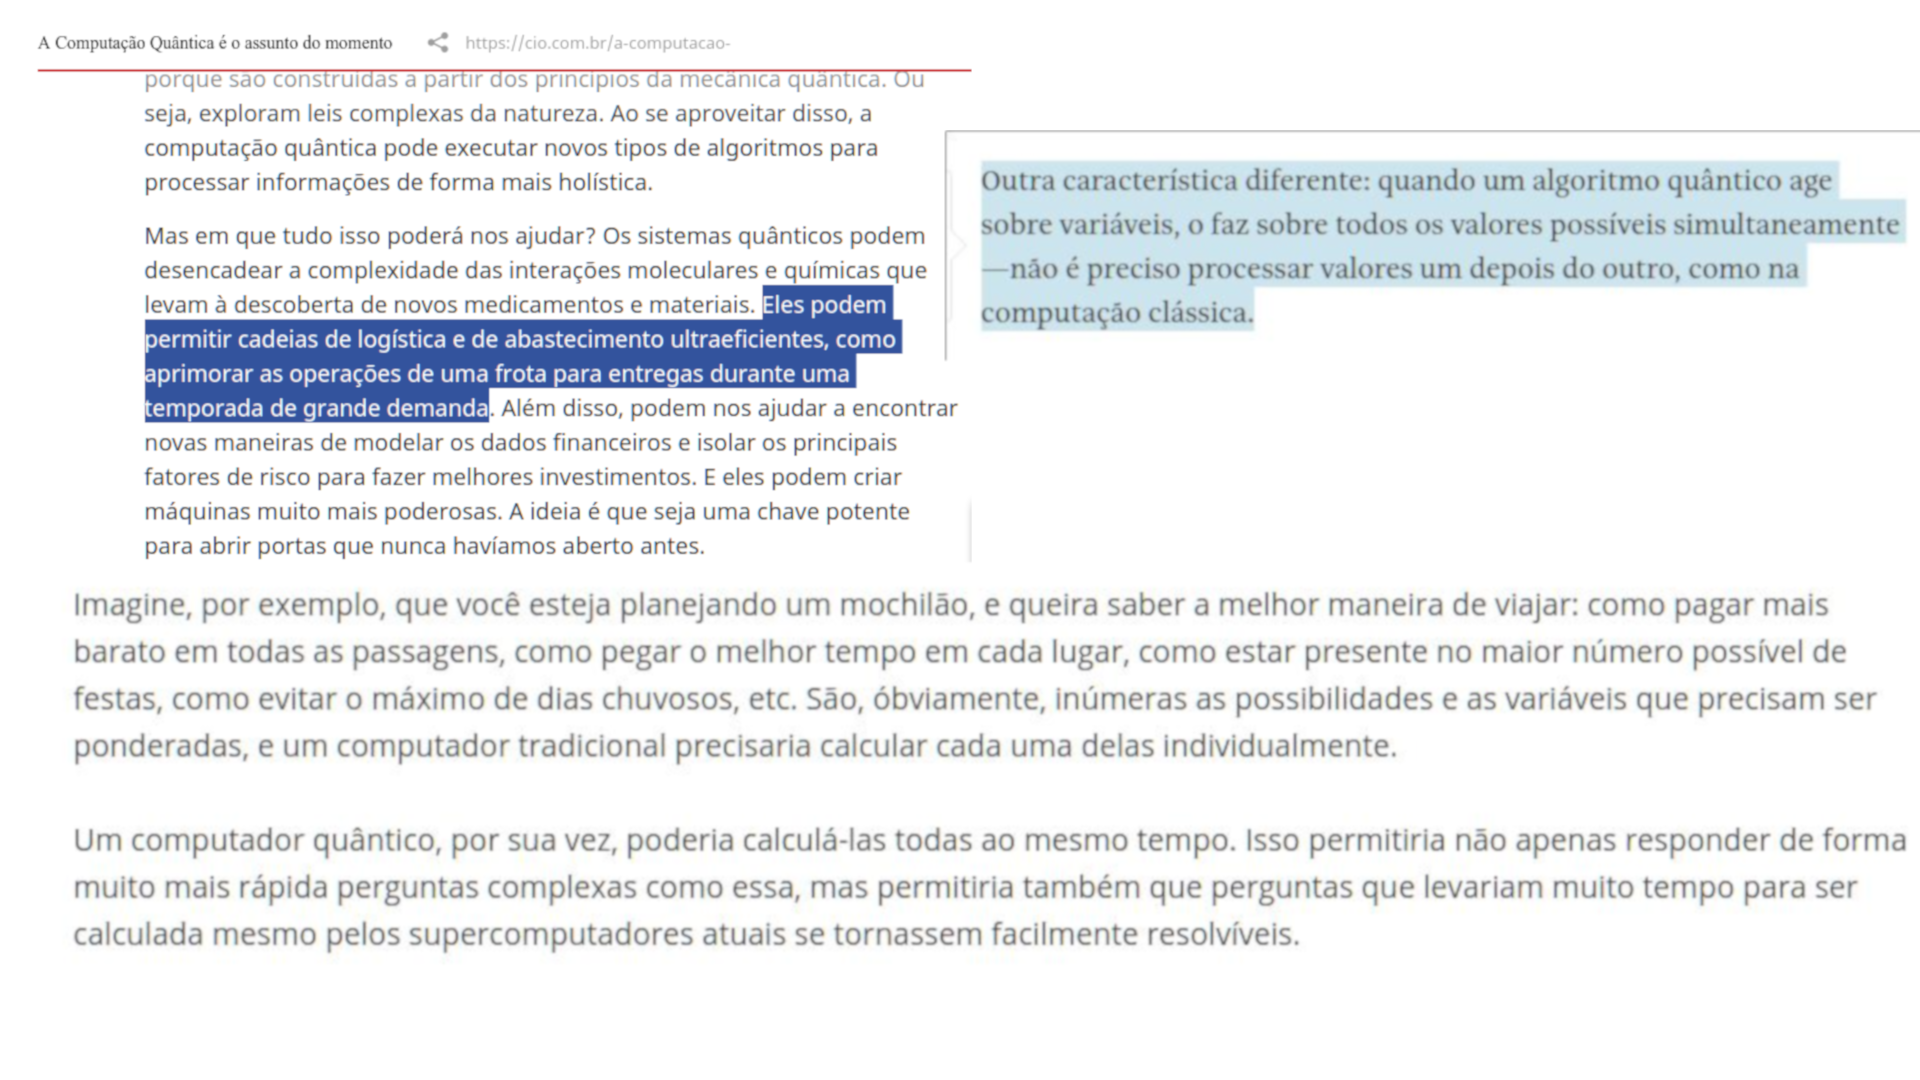
\includegraphics[width=1.0\textwidth]{lol.png}
\end{figure}
\end{frame}

\begin{frame}
\frametitle{Superposição}
\begin{itemize}
  \item A \textbf{Superposição quântica}: uma partícula pode assumir proporções entre dois estados.\\
  Ex: A polarização de um fóton (vertical ou horizontal). 
  \item A superposição quântica pode ser utilizada para representar informação binária: \textbf{qubit}.
  \item A computação quântica utiliza dados armazenados em qubits: 0 - 1 (qualquer proporção de ambos estados).
\end{itemize}
\end{frame}

\begin{frame}
\frametitle{Representação dos Qubits}
\begin{itemize}
  \item Os dois estados base de um qubit são representados pelos vetores

\begin{align}
\label{vet}
  \ket{0} \: = \begin{bmatrix} 
          1 \\ 
          0 \\ 
        \end{bmatrix}
  \:\text{e}\:
  \ket{1} \: = \begin{bmatrix} 
          0 \\ 
          1 \\ 
        \end{bmatrix}
\end{align}
Isso é conhecido como a notação de \textit{Dirac Ket} para vetores.
\item Para completamente representar o estado de um qubit são
  necessários dois números ($a, b$) \textbf{complexos} para descrever
  as duas proporções das duas bases:
\begin{align}
\label{amp}
  \Psi = a \ket{0} + b \ket{1}.
\end{align}
\end{itemize}
\end{frame}

\begin{frame}
\frametitle{Espaço de Estado de um Qubit}
\begin{itemize}
\item Utiliza-se a 2-norma:
  \begin{align}
    \label{sum1}
      |a|^2 + |b|^2 = 1
  \end{align}
\item Devido a restrição da equação \ref{sum1} os possíveis valores de um
  quibit se limitam uma equação de uma esfera de três dimensões.
\begin{figure}[h]
\label{bloch}
\centering
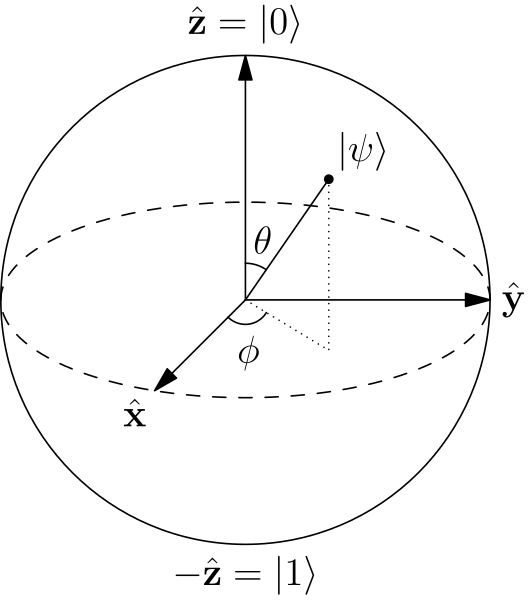
\includegraphics[width=0.25\textwidth]{bloch.png}
\end{figure}
\end{itemize}
\end{frame}

\begin{frame}
\frametitle{Operações em Qubits}
\begin{itemize}
  \item Operações em qubit são feitas por produtos de matrizes unitárias, também chamado
  de transformação unitária.
  \item Uma transformação de um qubit é uma translação no espaço de estado.
  \item O qubit $\ket{0}$ está no polo norte da Esfera de Bloch é
    levado para o seu equador, um estado de superposição, pelo produto
    na Equação \ref{trans}.
       \begin{align}
         \label{trans}
       \begin{bmatrix} 
                 \frac{1}{\sqrt{2}} & \frac{1}{\sqrt{2}}\\ 
                 \frac{1}{\sqrt{2}} & -\frac{1}{\sqrt{2}}\\ 
       \end{bmatrix}
         \cdot
       \begin{bmatrix} 
                 1 \\ 
                 0 \\ 
       \end{bmatrix}
         =
       \begin{bmatrix} 
                \frac{1}{\sqrt{2}} \\ 
                \frac{1}{\sqrt{2}} \\ 
       \end{bmatrix}
       \end{align}
  \item Aplicar uma segunda vez essa transformação levaria novamente para o qubit $\ket{0}$.
\end{itemize}
\end{frame}

\begin{frame}
\frametitle{Emaranhamento Quântico}
\begin{itemize}
  \item Um par (ou mais) de partículas tem o seu estado associados de
  maneira que não é possível descrever o estado de uma delas
  individualmente.
\item
  \begin{enumerate}
    \item Dois \textit{spins} ($A$ e $B$) emaranhados por
      seus campos magnéticos, ambos preparados no estado $\ket{0}$.
    \item O \textit{spin} $A$ é colocado na superposição
      $\frac{1}{\sqrt{2}} \ket{0} + \frac{1}{\sqrt{2}} \ket{1}$ por meio da
      aplicação de um campo magnético oscilante.
    \item Aplica-se outro campo magnético no \textit{spin} $B$ que vai nega-lo (mudar para
      $\ket{1}$) somente se o \textit{spin} $A$ estiver no estado $\ket{0}$.
    \item O \textit{spin} $B$ está numa superposição de $\ket{0}$ e $\ket{1}$,
      devido ao emaranhamento com o \textit{spin} $A$.\\
      O sistema final é uma superposição
      $\frac{1}{\sqrt{2}} \ket{01} + \frac{1}{\sqrt{2}} \ket{10}$.
  \end{enumerate}
  \item O emaranhamento quântico é a chave para o paralelismo quântico!
    \\ A computação de um qubit afeta o estado de outro qubit.
\end{itemize}
\end{frame}

\begin{frame}
\frametitle{Algoritmo Quântico}
\centering
\Large Vídeo!
\end{frame}

\section{Computabilidade}

\begin{frame}
\frametitle{Portas Quânticas 1}
\begin{itemize}
  \item Portas quânticas são análogas as portas lógicas binárias: operam
    em $n$ bits/qubits e dão algum bit/qubit de resposta.
  \item Portas quânticas não perdem informação: são reversíveis.
  \item Considera a porta AND clássica e a porta quântica C-NOT (Control-NOT):
    \begin{figure}[!htb]
    \label{andcnot}
    \begin{minipage}{.4\textwidth}
      \centering
      \begin{tabular}{|l l|ll|}
      \hline
      A & B & A & $A$ AND $B$  \\ \hline
      0 & 0 & 0 & 0            \\ \hline
      0 & 1 & 0 & 0            \\ \hline
      1 & 0 & 1 & 0            \\ \hline
      1 & 1 & 1 & 1            \\ \hline
      \end{tabular}
    \end{minipage}
    \begin{minipage}{0.4\textwidth}
      \centering
      \centering
      \begin{tabular}{|l l|ll|}
      \hline
      A & B & A & $A$ CNOT $B$ \\ \hline
      0 & 0 & 0 & 0            \\ \hline
      0 & 1 & 0 & 1            \\ \hline
      1 & 0 & 1 & 1            \\ \hline
      1 & 1 & 1 & 0            \\ \hline
      \end{tabular}
    \end{minipage}
      \caption{Portas AND e CNOT.}
    \end{figure}
\end{itemize}
\end{frame}

\begin{frame}
\frametitle{Portas Quânticas 2}
\begin{itemize}
  \item Portas lógicas quânticas de $n$ qubits são transformações unitárias
    representadas por matrizes de tamanho $2^n \times 2^n$. Por exemplo,
    a porta lógica quântica CNOT tem a matriz unitária da Equação
    \ref{macnot} e a matriz da Equação \ref{trans} é a porta quântica
    Hadamard (H).
    \begin{align}
      \label{macnot}
    \begin{bmatrix} 
    1 & 0 & 0 & 0 \\
    0 & 1 & 0 & 0 \\
    0 & 0 & 0 & 1 \\
    0 & 0 & 0 & 1
    \end{bmatrix}
    \end{align}
\end{itemize}
\end{frame}

\begin{frame}
\frametitle{Circuitos Quânticos 1}
\begin{itemize}
  \item Circuitos clássicos e quânticos (com as devidas restrições) são um modelo de computação.
  \item Um circuito quântico é uma sequência de portas lógicas quânticas que
    operam sobre uma entrada de $n$ qubits.
  \item  \cite{be:97} provou que Circuitos Quânticos (com as devidas restrições)
    representam um modelo Turing-Completo.
  \item Não é trivial simular primitivas simples como
    \textit{looping}, \textit{branching} e composição no contexto de
    Máquinas de Turing Quânticas, pois as leis da Mecânica Quântica
    impõem restrições difíceis, como observar uma informação implica
    no colapso do seu estado.
\end{itemize}
\end{frame}

\begin{frame}
\frametitle{Circuitos Quânticos 2}
\begin{itemize}
  \item \textit{Conjunto universal de portas quânticas}
    (CUPQ) é um conjunto portas quânticas capaz de construir circuitos
    que representam tudo que um computador quântico pode fazer.
  \item Foi demostrado por \cite{shi:03} que as portas Toffoli e
    Hadamard são um CUPQ.
  \item Foi demonstrado por \cite{da:06} que qualquer CUPQ pode
    ser simulado por outro CUPQ em tempo polinomial.
\end{itemize}
\end{frame}

\section{Classes de Problemas}
\begin{frame}
  \frametitle{Classe de Problemas na Computação Tradicional}
  \begin{itemize}
  \item NP \textbf{(nondeterministic polynomial time)}:
    Problemas de decisão verificáveis em tempo polinomial.\\ \small{Eficientes no
    modelo computacional ``Máquina de Turing Não-Determinista''}.
    \item P: Problemas de decisão computáveis em tempo polinomial.\\ \small{Eficientes no
    modelo computacional ``Máquina de Turing Determinista''}.
  \end{itemize}
  \begin{figure}[h]
    \label{classpnp}
    \centering
    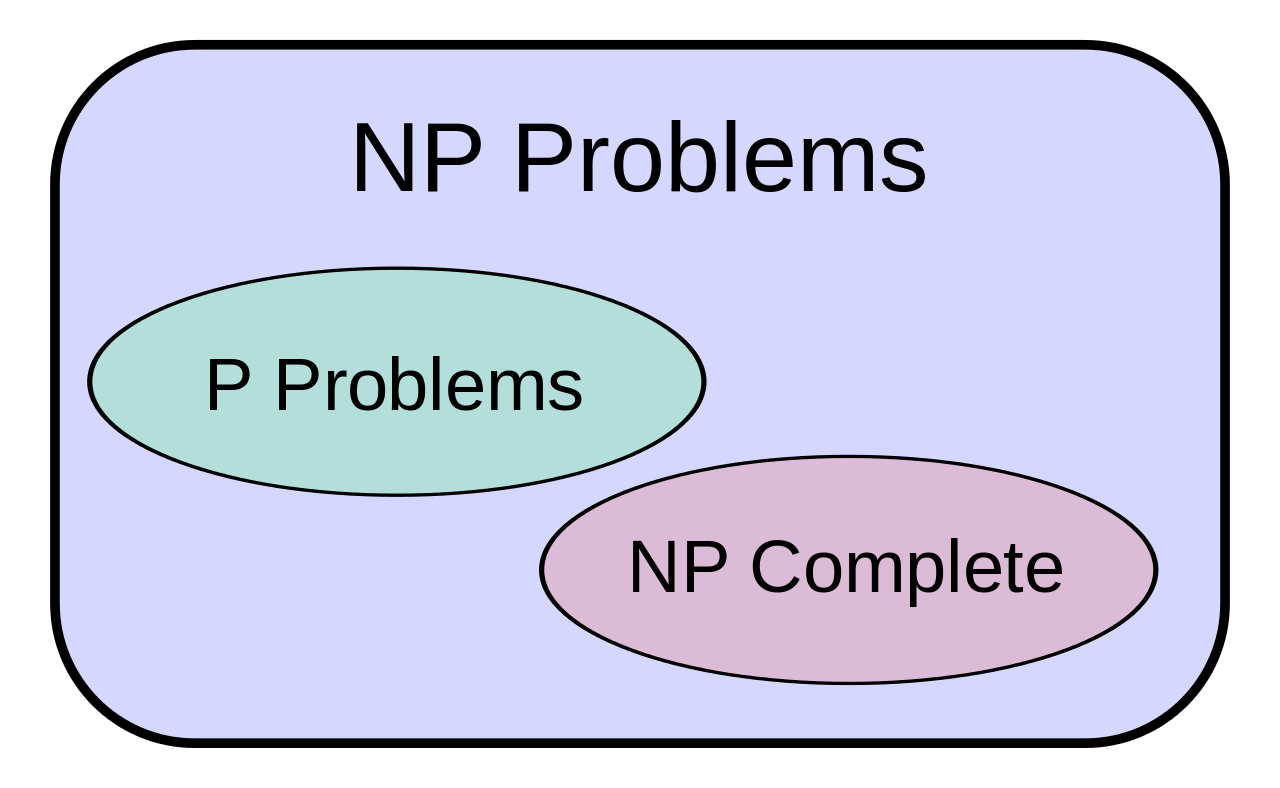
\includegraphics[width=0.45\textwidth]{classpnp.png}
  \end{figure}
  \centering{\textbf{P vs NP}}\\
  Exemplos de problemas: SAT, Caixeiro viajante...
\end{frame}

\begin{frame}
\frametitle{Classe Probabilística BPP} 
\begin{itemize}
  \item A classe BPP (\textit{Bounded-Error Probabilistic
      Polynomial-Time}): Polinomial por uma Máquina de Turing Probabilística (com um
    mecanismo de aleatoriedade).
  \item Somente é aceitável no máximo $1/3$ de chance de fornecer a
  resposta errada (seja sim ou não).
  \item A classe BPP funciona como um análogo probabilístico da classe P.
  \item A verificação de primalidade: BPP $\rightarrow$ P.
\end{itemize}
\end{frame}

\begin{frame}
\frametitle{Classe Quântica BQP} 
\begin{itemize}
  \item A classe de problemas resolvidos de maneira eficiente por
  computadores quânticos é a BQP (\textit{Bounded-Error Quantum
    Polynomial-Time}).
  \item Assim como a classe BPP, a classe BQP requer no máximo $1/3$ de
  chance de erro.
  \item Definida por Circuitos Quânticos.
  \item O número de qubits permitidos no circuito deve ser polinomial
    ao tamanho do problema.\\ O algoritmo de Shor para
    fatoração de números primos de $n$-bits requer um circuito de
    $2n$-qubits.
\end{itemize}
\end{frame}

\begin{frame}
\frametitle{Relação Entre as Classes} 
\begin{itemize}
  \item BPP $\subseteq$ BQP, pois como fonte de aleatoriedade basta utilizar a porta Hadamard.
  \item A classe PP é similar a BPP, mas com requisito de probabilidade
  difícil o suficiente para não ser possível aumentar a chance de
  acerto ao rodar o algoritmo várias vezes.
  \item A Classe PSPACE: problemas resolvidos com espaço polinomial,
  mas com tempo ilimitado.
  \item P $\subseteq$ BPP $\subseteq$ BQP $\subseteq$ PP $\subseteq$ PSPACE.
\end{itemize}
\end{frame}

\begin{frame}
\frametitle{\small{O Maior Problema da Teoria da Complexidade Quântica}} 
\begin{centering}
\large{Computadores quânticos são mais eficientes que computadores probabilísticos clássicos?}
\end{centering}
\begin{itemize}
  \item BPP $\not =$ BQP
  \item A evidência mais popular que isso é verdade é o algoritmo
  quântico Shor e o fato que até hoje ninguém descobriu um eficiente
  algoritmo probabilístico que realiza o mesmo trabalho.
\end{itemize}
\end{frame}

\begin{frame}
\frametitle{Classes com Oráculos} 
\begin{itemize}
  \item Não há relação direta entre a classe NP e
  as classe probabilística BQP.
  \item Ao menos, sabe-se que a classe BPP está contida na classe
  NP$^{\text{NP}}$ (NP com um oráculo NP).
  \item Há a classe PH (Polynomial Hierarchy) que contém todos as
  classes com tempo polinomial estendidas com máquinas oráculos,
  inclusive NP e BPP.
  \item O papel do oráculo é funcionar como uma espécie de
  medida de dificuldade do problema, quanto mais um algoritmo precisa
  consultar o oráculo, mais difícil é o problema.
  \item PH é uma generalização (e um superconjunto) da classe NP. 
\end{itemize}
\end{frame}

\begin{frame}
\frametitle{BQP $\subseteq$ PH?} 
\begin{itemize}
  \item BQP está contida em PH?\\
   Isso questiona se há problemas somente tratáveis por um
   computador quântico, mesmo que P = NP
  \item Computadores quânticos são um caso a parte na Teoria da
   Complexidade?
  \item Em 2009 Aaronson introduziu o problema da ``fourrelação'' e
   demostrou estar em BQP \cite{aa:09}.
  \item Em Maio de 2018 \cite{ra:18} demostraram que esse problema não
   está em PH.
  \item Uma computador quântico precisa de apenas uma consulta a um
   oráculo para resolver esse problema, enquanto um computador
   clássico não é capaz de resolve-lo de maneira eficiente, mesmo com
   um número ilimitado de consultas.
\end{itemize}
\end{frame}

\begin{frame}
  \frametitle{Ilha da Complexidade Quântica}
    \begin{figure}[h]
    \label{notph}
    \centering
    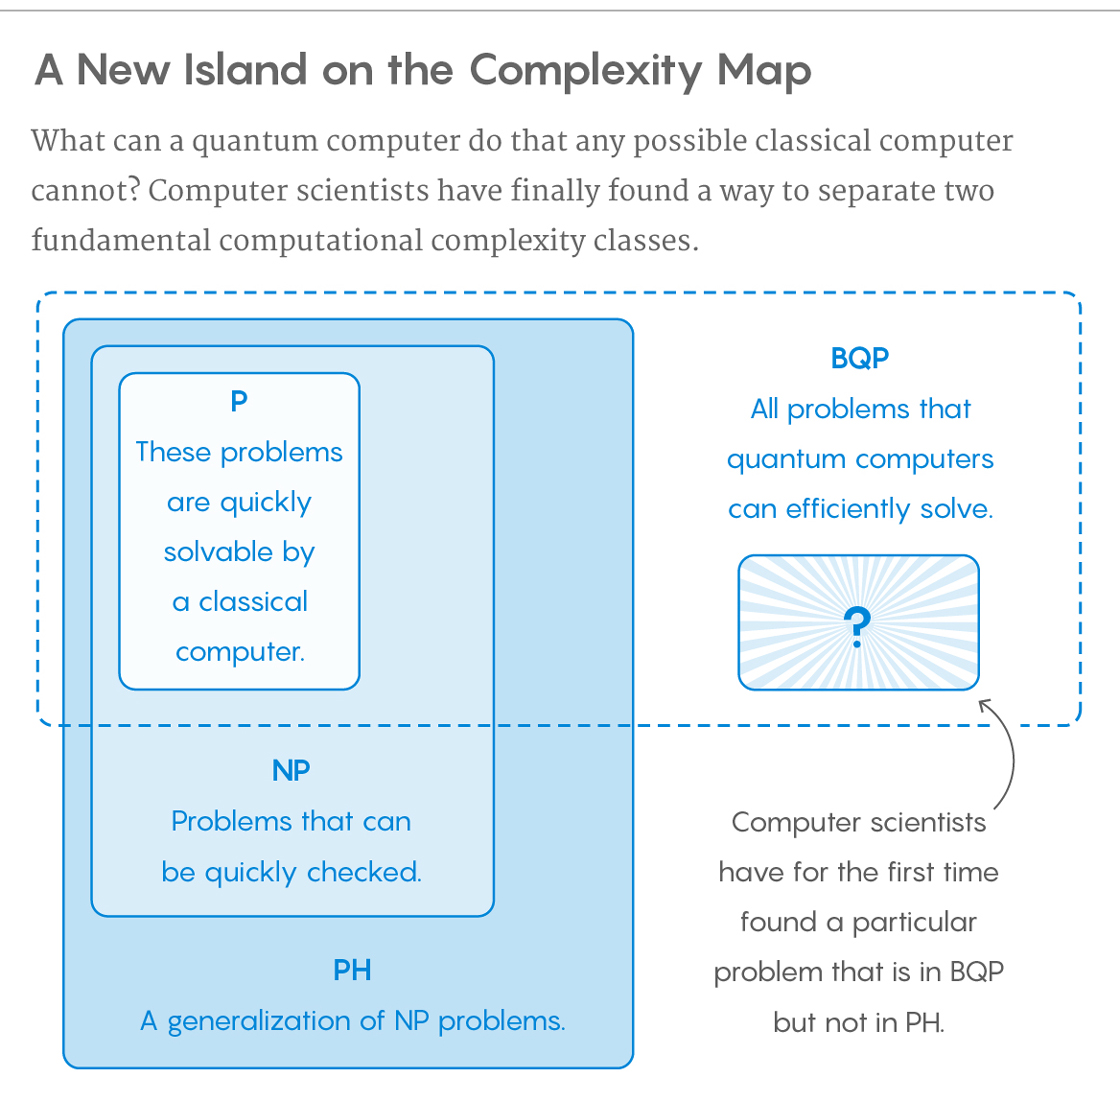
\includegraphics[width=0.6\textwidth]{island.jpg}
    \caption{Ilha de complexidade BQP. Fonte: QuantaMagazine.org.}
    \end{figure}
\end{frame}

\begin{frame}
\frametitle{\textit{Computational Complexity-Theoretic Church–Turing Thesis}} 
\begin{itemize}
  \item Esse novo resultado inválida a \textit{computational
    complexity-theoretic Church–Turing thesis}
  \item Proposto por \cite{be:97}, que diz que uma Máquina de Turing
  Probabilística pode simular em tempo polinomial qualquer outro
  modelo de computação.
  \item Algoritmos quânticos são eficientes em tarefas que
  algoritmos probabilísticos não são.
\end{itemize}
\end{frame}

\begin{frame}
\frametitle{NP-Completude e Computação Quântica} 
\begin{itemize}
  \item Erroneamente muitas pessoas ou sites/revistas de notícias
  anunciam que a computação quântica é capaz de resolver de maneira
  eficiente problemas NP-Completos.
  \item O status de NP $\subset$ BQP é desconhecido.
  \item É sabido uma separação por oráculo de NP $\not \subset$ BQP:
    suponha um problema com espaço de busca de tamanho $2^n$ de
  possíveis soluções e um oráculo que decide se a uma possível solução
  é a procurada.
  \item Num computador normal, no pior dos casos, é necessário $2^n$
  consultas no oráculo.
  \item Por meio do algoritmo de Groover \cite{gr:96} é possível
  encontrar a resposta em até $2^{n/2}$ consultas.
\end{itemize}
\end{frame}

\begin{frame}
\frametitle{Speed-up da Computação Quântica} 
\begin{itemize}
  \item O \textit{speed-up} da computação quântica para problemas de
    busca genéricos e não estruturados é quadrático.
  \item Não é conhecido como fazer \textit{speed-up} exponencial para esse tipo de problema.
  \item Speed-up quadrático não é suficiente para um NP-Completo ser polinomial num computador
    quântico.
\end{itemize}
\end{frame}

\begin{frame}
  \frametitle{Resumindo...}
  \begin{itemize}
  \item Não sabemos como resolver de maneira eficiente problemas
    NP-Completos num computador quântico. 
  \item Não tem essa de testar todas as possibilidades ao mesmo tempo.
  \end{itemize}
\end{frame}

\begin{frame}[allowframebreaks, noframenumbering]
  \frametitle{Referências}
   \bibliographystyle{apalike}
  \bibliography{sbc-template}
\end{frame}

\end{document}
%%% Local Variables:
%%% mode: latex
%%% TeX-master: t
%%% End:
